应用程序通常是包含主机代码和设备代码的组合。有一些类成员允许我们提交设备代码,并且这些工作分发机制是提交到设备执行的唯一方式,以便我们轻松地区分设备代码和主机代码。\par

本章的其余部分将介绍一些工作分发机制,目的是帮助了解和辨别在主机处理器上本机执行的设备代码和主机代码之间的区别。\par

\hspace*{\fill} \par %插入空行
\textbf{任务图}

SYCL执行模型中的一个基本概念是节点图。图中的每个节点(工作单元)都包含一个在设备上执行的操作,其中最常见的操作是数据并行设备的内核调用。图2-17展示了一个有四个节点的示例图,其中每个节点都可以看作是一个设备内核。\par

图2-17中的节点具有依赖边,定义了节点的工作何时开始。依赖边最常见的是数据依赖项自动生成的,尽管也可以在需要时手动添加额外的依赖项,例如:图中的节点B与节点A有一条依赖边,这条边意味着节点A必须在B开始前完成执行,然后将结果数据放在节点B的设备上。运行时控制依赖项的解析和节点执行的触发,与主机程序的完全异步。定义应用程序的节点图在本书中称为任务图,并在第3章中进行更详细的介绍。\par

\hspace*{\fill} \par %插入空行
图2-17 任务图定义了要在一个或多个设备上执行的操作(与主机程序异步执行),还定义了何时可以安全执行某个操作的依赖项
\begin{center}
	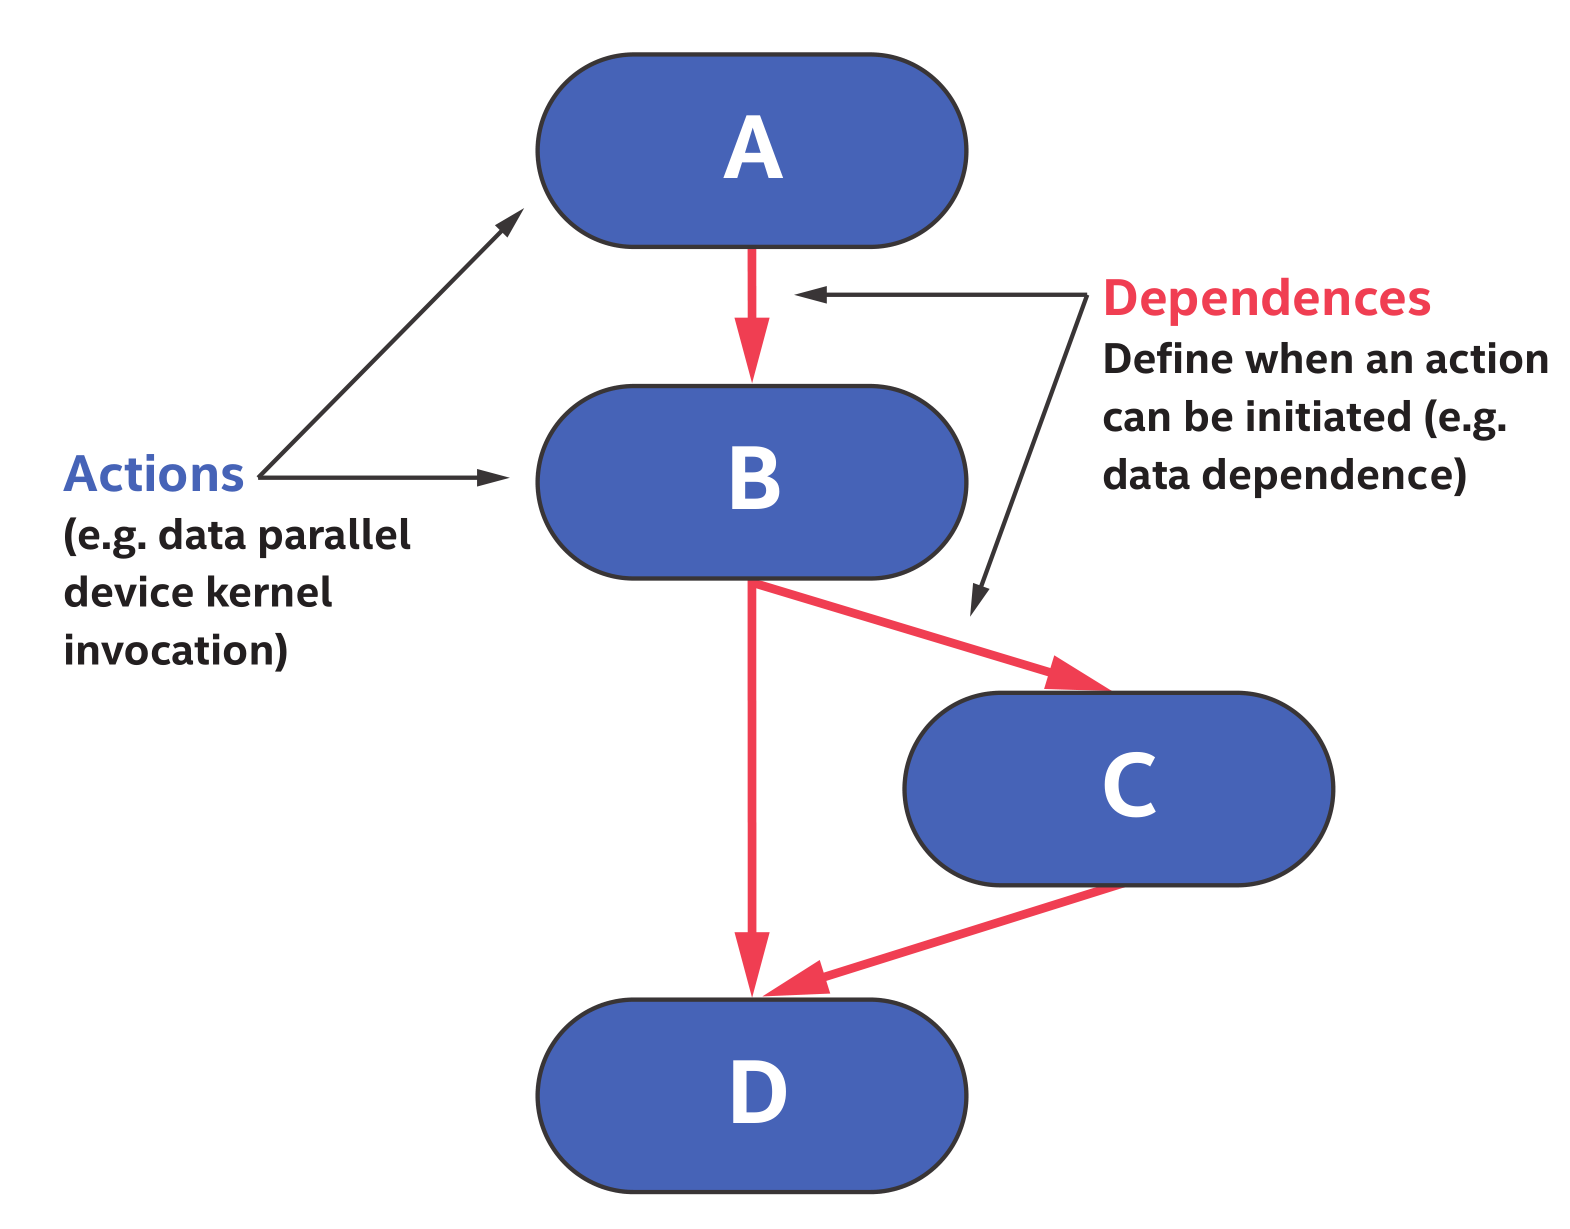
\includegraphics[width=0.8\textwidth]{content/chapter-2/images/10}
\end{center}

\hspace*{\fill} \par %插入空行
图2-18 提交设备代码
\begin{center}
	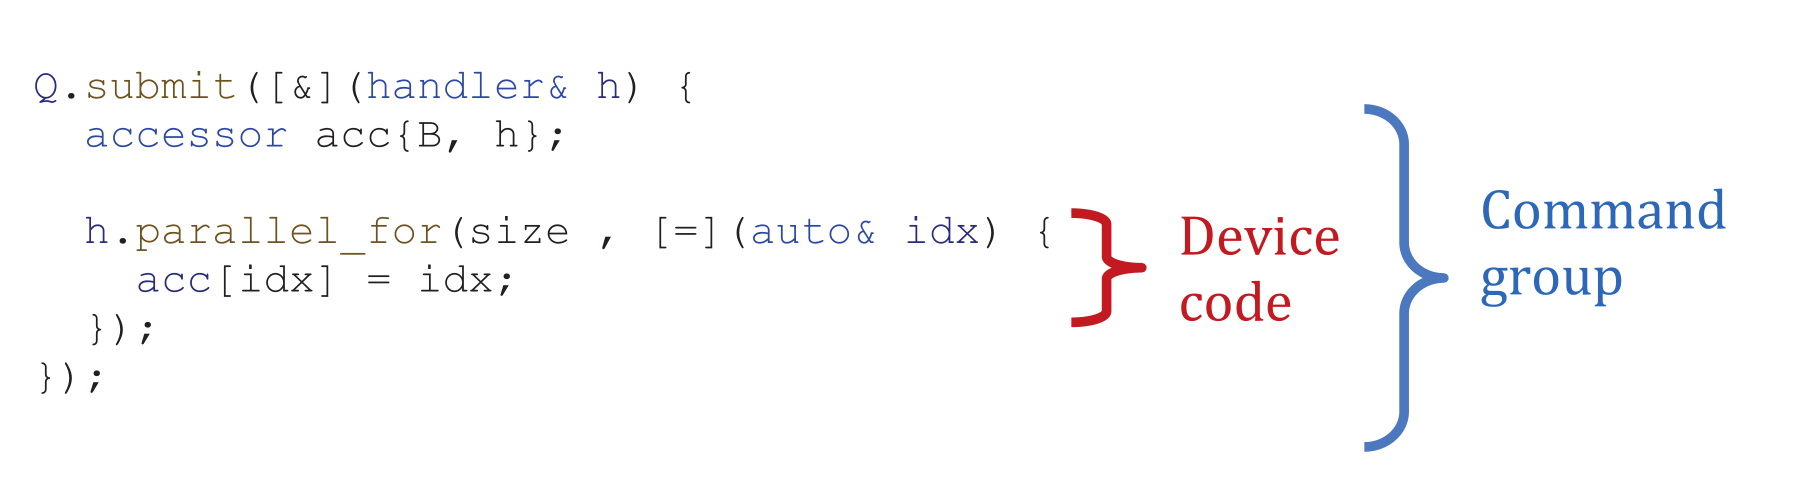
\includegraphics[width=0.8\textwidth]{content/chapter-2/images/11}
\end{center}

\hspace*{\fill} \par %插入空行
\textbf{设备代码在哪里?}

有多种机制可以在设备上执行代码,但需要例子展示了如何识别这些代码。即使示例中的模式看上去很复杂,但其模式在所有设备代码定义中都是相同的,因此就成为了第二特性。\par

图2-18中定义为lambda,作为最后一个参数传递给parallel\_for的代码,这个lambda表达式就是要在设备上执行的设备代码。并行的parallel\_for中可以区分设备代码和主机代码。parallel\_for是设备调度机制的一个小集合,都是handler类的成员,其定义了要在设备上执行的代码。图2-19给出了handler类的定义。\par

\hspace*{\fill} \par %插入空行
图2-19 handler类中成员函数的定义
\begin{lstlisting}[caption={}]
class handler { 
public:
	// Specify event(s) that must be complete before the action 
	// defined in this command group executes.
	void depends_on(std::vector<event>& events);
	
	// Guarantee that the memory object accessed by the accessor
	// is updated on the host after this action executes.
	template <typename AccessorT>
		void update_host(AccessorT acc);
	
	// Submit a memset operation writing to the specified pointer.
	// Return an event representing this operation.
	event memset(void *ptr, int value, size_t count); 
	
	// Submit a memcpy operation copying from src to dest.
	// Return an event representing this operation.
	event memcpy(void *dest, const void *src, size_t count);
	
	// Copy to/from an accessor and host memory.
	// Accessors are required to have appropriate correct permissions.
	// Pointer can be a raw pointer or shared_ptr.
	template <typename SrcAccessorT, typename DestPointerT>
		void copy(SrcAccessorT src, DestPointerT dest);
		
	template <typename SrcPointerT, typename DestAccessorT>
		void copy(SrcPointerT src, DestAccessorT dest);
	
	// Copy between accessors.
	// Accessors are required to have appropriate correct permissions.
	template <typename SrcAccessorT, typename DestAccessorT>
		void copy(SrcAccessorT src, DestAccessorT dest);
	
	// Submit different forms of kernel for execution.
	template <typename KernelName, typename KernelType>
		void single_task(KernelType kernel);
		
	template <typename KernelName, typename KernelType, int Dims>
		void parallel_for(range<Dims> num_work_items, 
							KernelType kernel); 
							
	template <typename KernelName, typename KernelType, int Dims>
		void parallel_for(nd_range<Dims> execution_range, 
							KernelType kernel);
							
	template <typename KernelName, typename KernelType, int Dims>
		void parallel_for_work_group(range<Dims> num_groups, 
							KernelType kernel);
							
	template <typename KernelName, typename KernelType, int Dims>
		void parallel_for_work_group(range<Dims> num_groups,
									range<Dims> group_size, 
									KernelType kernel);
};
\end{lstlisting}

除了调用handler类的成员来提交设备代码之外,还有允许提交工作的queue类成员。图2-20表示queue类成员是某些模式的快捷方式,我们将在以后的章节中看到这些快捷方式的使用。\par

\hspace*{\fill} \par %插入空行
图2-20 queue类中成员函数的定义,该成员函数充当handler类中等效函数的快捷方式
\begin{lstlisting}[caption={}]
class queue {
public:
	// Submit a memset operation writing to the specified pointer.
	// Return an event representing this operation.
	event memset(void *ptr, int value, size_t count)
	
	// Submit a memcpy operation copying from src to dest.
	// Return an event representing this operation.
	event memcpy(void *dest, const void *src, size_t count);
	
	// Submit different forms of kernel for execution.
	// Return an event representing the kernel operation.
	template <typename KernelName, typename KernelType>
		event single_task(KernelType kernel);
		
	template <typename KernelName, typename KernelType, int Dims>
		event parallel_for(range<Dims> num_work_items, 
						KernelType kernel); 
						
	template <typename KernelName, typename KernelType, int Dims>
		event parallel_for(nd_range<Dims> execution_range, 
						KernelType kernel); 
						
	// Submit different forms of kernel for execution. 
	// Wait for the specified event(s) to complete 
	// before executing the kernel. 
	// Return an event representing the kernel operation.
	template <typename KernelName, typename KernelType>
		event single_task(const std::vector<event>& events, 
						KernelType kernel);
						
	template <typename KernelName, typename KernelType, int Dims>
	event parallel_for(range<Dims> num_work_items, 
						const std::vector<event>& events, 
						KernelType kernel);
	
	template <typename KernelName, typename KernelType, int Dims>
		event parallel_for(nd_range<Dims> execution_range, 
						const std::vector<event>& events, 
						KernelType kernel);
};
\end{lstlisting}

\hspace*{\fill} \par %插入空行
\textbf{行动机制}

图2-18中的代码包含一个parallel\_for,定义了要在设备上执行的工作。parallel\_for位于提交给队列的命令组(CG)中,队列定义了要在其上执行工作的设备。在命令组中,有两类代码:\par

\begin{enumerate}
	\item \textbf{一项行动只有一次调用},设备代码将排队等待执行,或执行手动内存操作(如复制)。
	\item \textbf{主机代码}会设置依赖项,这些依赖项定义了代码时何时开始执行(1)是安全的,例如:创建缓冲区的访问器(在第3章介绍)。
\end{enumerate}

handler类包含一组成员函数,这些函数定义了在执行任务图节点时要执行的操作。图2-21对这些操作进行了总结。\par

图2-21中只有一个动作可以在命令组中调用(调用多个是错误的),而且每个提交调用只能将一个命令组提交到一个队列中。这样,图2-21中的单个操作存在于每个任务图节点上,当节点依赖关系满足,且运行时安全时,就可以执行了。\par

\begin{tcolorbox}[colback=red!5!white,colframe=red!75!black]
	命令组中只能有一个操作,例如:内核启动或显式内存操作。
\end{tcolorbox}

代码是异步执行的,这就是主机程序一部分运行在CPU上和满足依赖关系时运行的设备代码之间的关键区别。命令组通常包含来自每种类别的代码,其中的代码定义了作为宿主程序运行的依赖项(以便运行时知道这些依赖项是什么),以及在满足这些依赖项后在将要运行的设备代码。\par

图2-21 调用设备代码或执行显式内存的操作
\begin{table}[]
	\begin{tabular}{|m{32mm}|c|p{6cm}|}
		\hline
		\multicolumn{1}{|l|}{\textbf{工作类型}}            & \multicolumn{1}{|c|}{\textbf{行为(handler类的成员函数)}} & \textbf{总结}                                                                                                                                   \\ \hline
		\multirow{3}{10em}{\textbf{设备代码执行}}     & single\_task                                                 & 执行一个设备函数的单例                                                                                                   \\ \cline{2-3} 
		& parallel\_for                                                & 有多种形式可用来启动不同组合的设备代码                                                       \\ \cline{2-3} 
		& parallel\_for\_work\_group                                   & 使用层次并行启动一个内核,在第4章介绍                                                                       \\ \hline
		\multirow{3}{10em}{\textbf{显式内存操作}} & copy                                                         & 访问器、指针和/或shared\_ptr指定的位置之间复制数据。复制作为DAG的一部分发生,包括依赖性跟踪。 \\ \cline{2-3} 
		& update\_host                                                 & 触发缓存对象在主机端的备份更新。                                                                                          \\ \cline{2-3} 
		& fill                                                         & 将内存中的数据初始化为指定的值。                                                                                               \\ \hline
	\end{tabular}
\end{table}

\hspace*{\fill} \par %插入空行
图2-22 提交设备代码
\begin{center}
	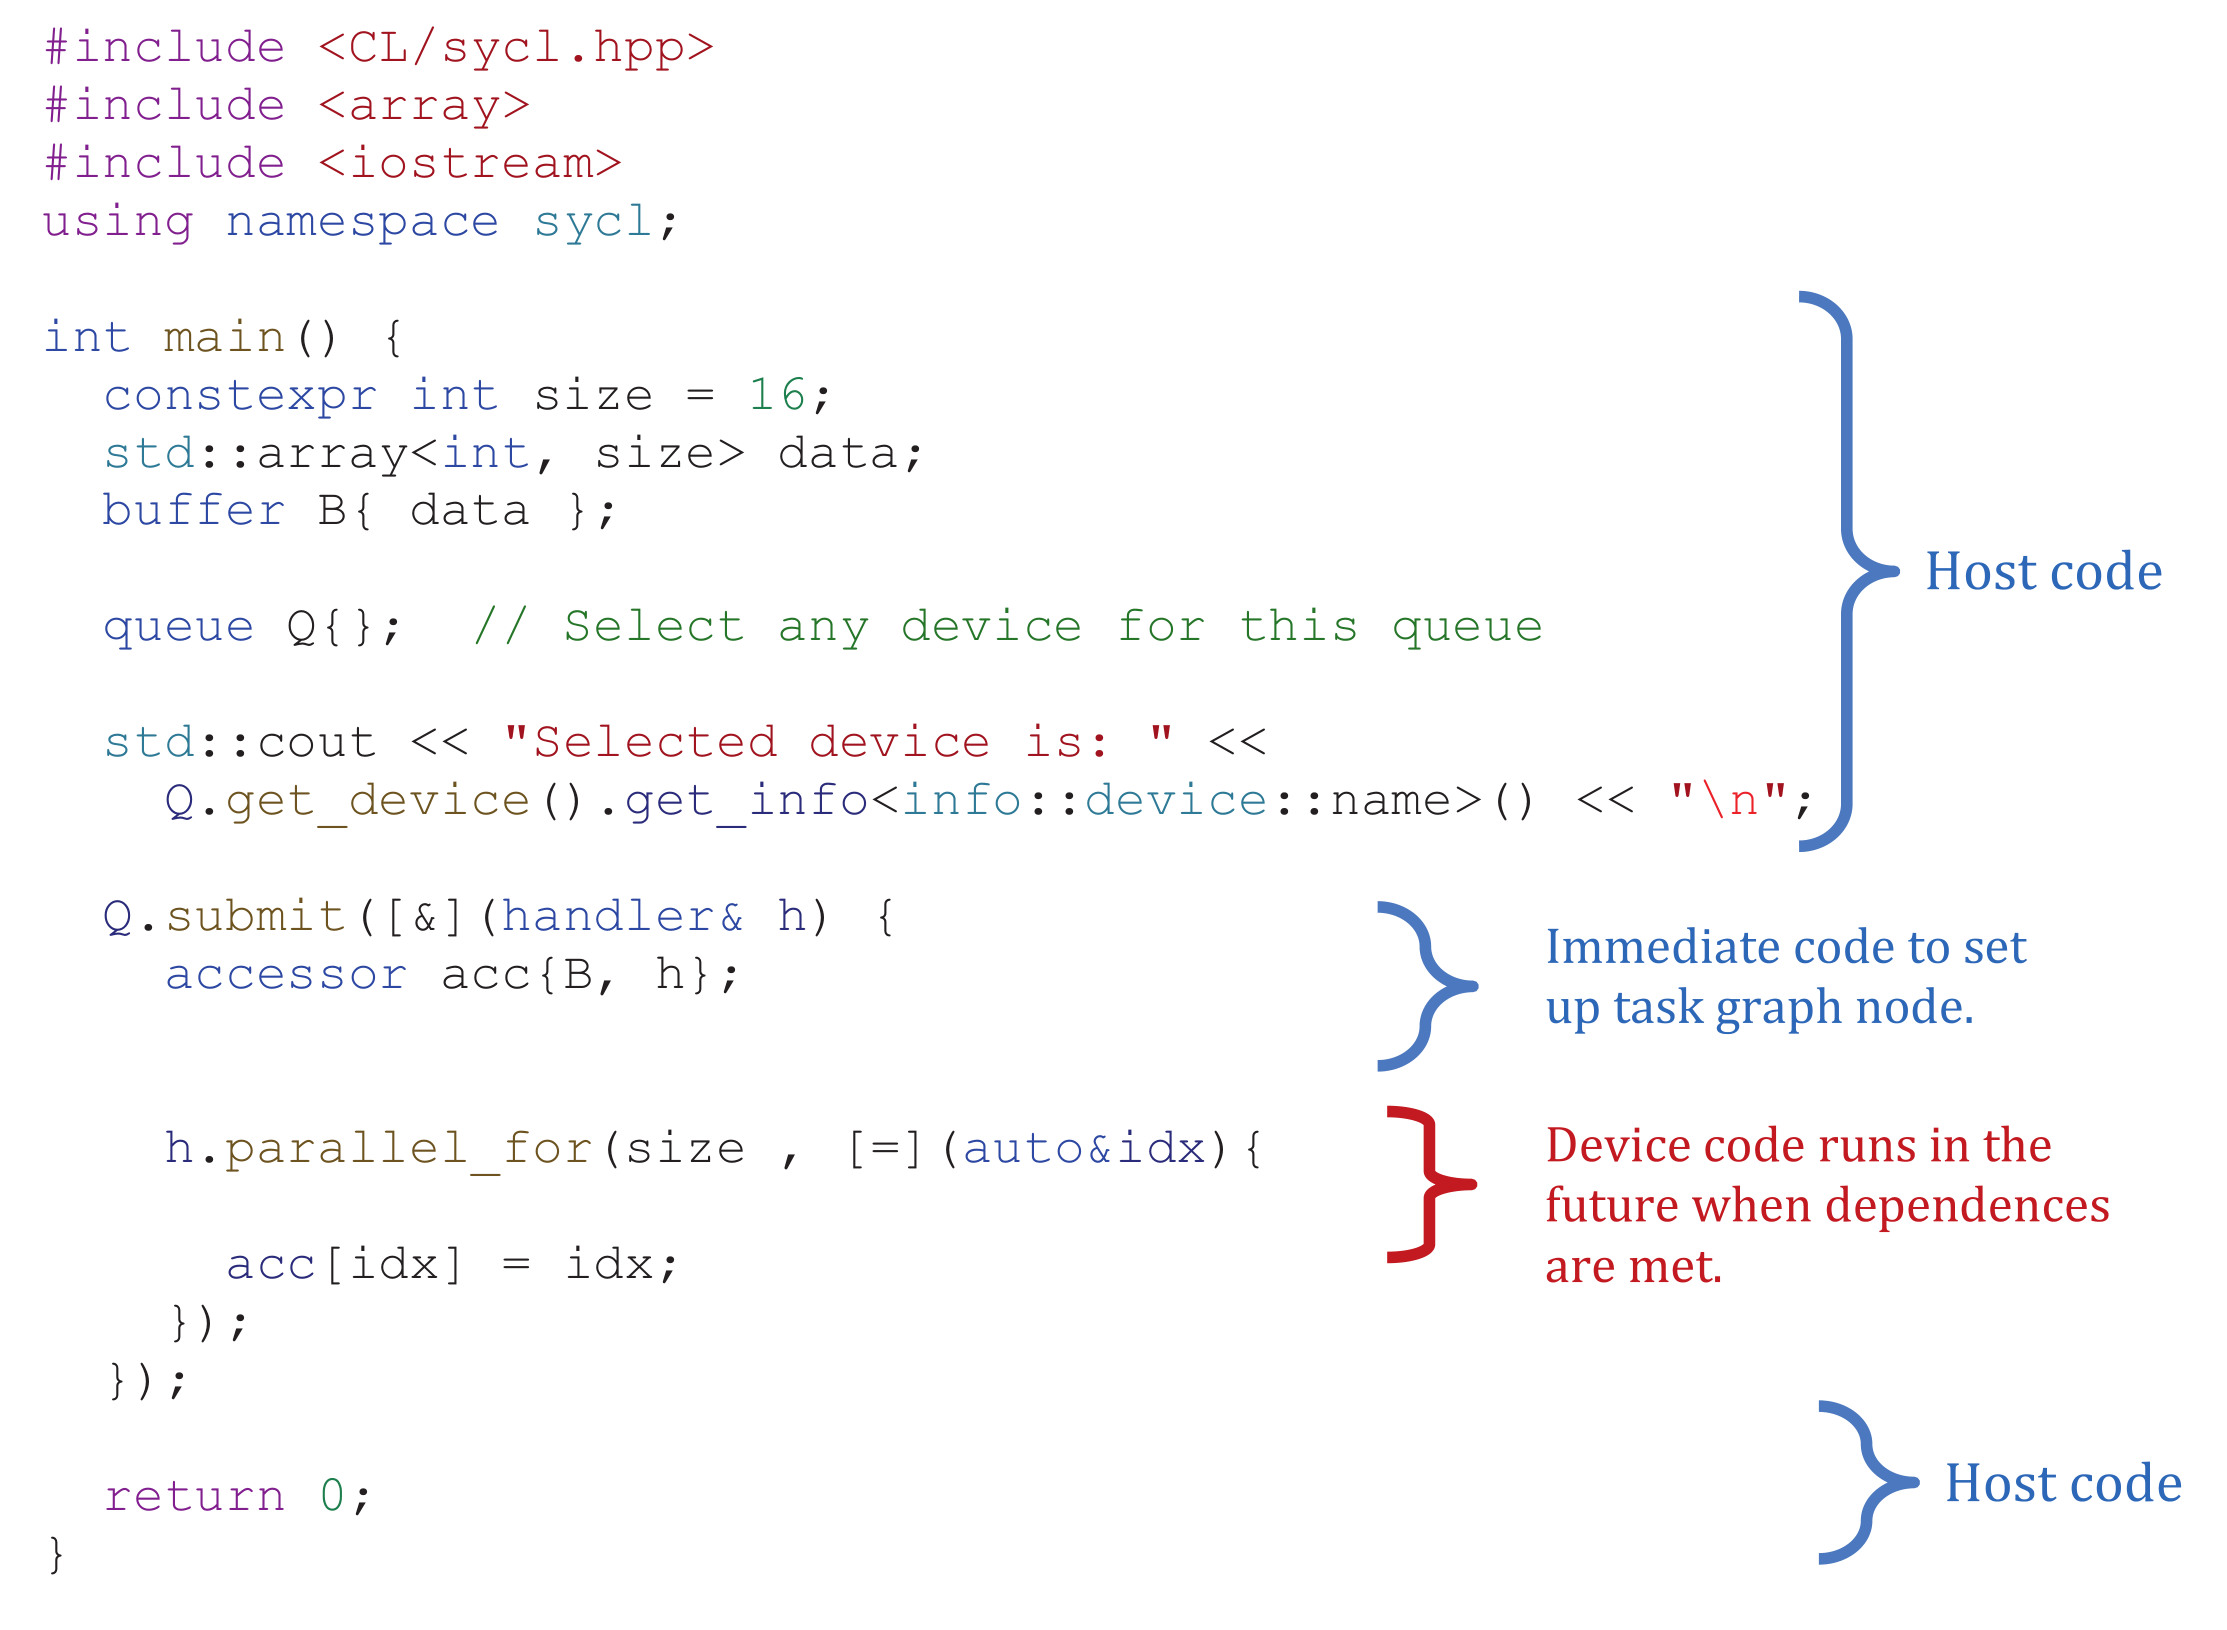
\includegraphics[width=0.9\textwidth]{content/chapter-2/images/12}
\end{center}

图2-22中有三类代码:\par

\begin{enumerate}
	\item 主机代码:驱动应用程序,包括创建和管理数据缓冲区,并向队列提交任务,在任务图中形成新的节点,以便异步执行。
	\item 命令组中的主机代码:代码在执行主机代码的处理器上运行,并在submit返回前执行,例如:代码通过创建访问器来设置节点依赖关系。任何的CPU代码都可以在这里执行,但最佳实践是将其限制为配置节点依赖关系的代码。
	\item 动作机制:图2-21中列出的任何动作都可以包含在命令组中,它定义了在节点满足要求(由(2)设置)时要异步执行的工作。
\end{enumerate}

为了理解应用程序中的代码何时会运行,注意图2-21中列出的启动设备代码的动作,以及图2-21中列出的显式内存操作,都会在DAG节点依赖满足时异步执行。所有其他代码会作为主程序的一部分立即运行,如同典型的C++代码那样。\par

\hspace*{\fill} \par %插入空行
\textbf{后备队列机制}

通常,命令组在提交的命令队列上执行。某些情况下,命令组提交到队列会失败(例如,当请求的工作大小超过设备的限制),或者成功提交的操作无法执行(例如,当硬件设备发生故障)。要处理这种情况,可以为执行的命令组指定一个后备队列。不过,不推荐这种错误管理方式,因为它的可控性太少,更建议捕捉和管理这些问题,会在第5章中进行介绍。这里简要介绍下后备队列,因为有些人喜欢这种方式,其在SYCL中比较有名。\par

这种类型的回退,适用于设备队列会提交失败的机器,但这不是解决加速器不存在问题的机制。在没有GPU设备的系统上,图2-23中的程序会在Q声明(尝试构造)处抛出一个错误,指示“所请求类型的设备不可用”。\par

基于现有设备的后备将在第12章中进行介绍。\par

\hspace*{\fill} \par %插入空行
图2-23 后备队列的例子
\begin{lstlisting}[caption={}]
#include <CL/sycl.hpp>
#include <array>
#include <iostream>
using namespace sycl;

int main() {
	constexpr int global_size = 16;
	constexpr int local_size = 16;
	buffer<int,2> B{ range{ global_size, global_size }};
	
	queue gpu_Q{ gpu_selector{} };
	queue host_Q{ host_selector{} };
	
	nd_range NDR {
		range{ global_size, global_size },
		range{ local_size, local_size }};
	
	gpu_Q.submit([&](handler& h){
		accessor acc{B, h};
		h.parallel_for( NDR , [=](auto id) {
			auto ind = id.get_global_id();
			acc[ind] = ind[0] + ind[1];
		});
	}, host_Q); /** <<== Fallback Queue Specified **/

	host_accessor acc{B};
	for(int i=0; i < global_size; i++){
		for(int j = 0; j < global_size; j++){
			if( acc[i][j] != i+j ) {
				std::cout<<"Wrong result\n";
				return 1;
	} } }
	std::cout<<"Correct results\n";
	return 0;
}
\end{lstlisting}

由于工作组请求的大小,图2-23所示的代码会在一些GPU上执行失败。我们可以指定一个辅助队列作为submit函数的参数,如果命令组无法进入主队列,则使用这个辅助队列(本例中是主机设备)。\par

\begin{tcolorbox}[colback=red!5!white,colframe=red!75!black]
通过向提交调用传递辅助队列来启用后备队列。不过,建议对捕获初始错误并进行处理,而不是使用提供较少可控性的后备队列机制。
\end{tcolorbox}
